\documentclass[12pt, titlepage]{article}

\usepackage[a4paper,margin=1in,footskip=0.25in]{geometry}
\usepackage{indentfirst}
\usepackage{xcolor}
\usepackage{tabularx}
\usepackage{booktabs}
\usepackage{hyperref}
\usepackage{listings}
\usepackage{graphicx}
\usepackage[round]{natbib}
\usepackage{multirow}
\hypersetup{
    colorlinks,
    citecolor=black,
    filecolor=black,
    linkcolor=black,
    urlcolor=blue
}
\usepackage[round]{natbib}

\newcounter{acnum}
\newcommand{\actheacnum}{AC\theacnum}
\newcommand{\acref}[1]{AC\ref{#1}}

\newcounter{ucnum}
\newcommand{\uctheucnum}{UC\theucnum}
\newcommand{\uref}[1]{UC\ref{#1}}

\newcounter{mnum}
\newcommand{\mthemnum}{M\themnum}
\newcommand{\mref}[1]{M\ref{#1}}

%%%%%%%%%%%%%
%%% title %%%
%%%%%%%%%%%%%

\title{\textbf{SE 3XA3: Module Guide}\\Lines Per Minute (lpm)}

\author{Team \#16, Lines Per Minute (lpm)\\
Jay Mody - modyj - 400195508\\
Jessica Lim - limj31 - 400173669\\
Maanav Dalal - dalalm1 - 400178115\\
}

\date{\today}

\begin{document}

\maketitle
\begin{table}[hp]
\caption{Revision History} \label{TblRevisionHistory}
\begin{tabularx}{\textwidth}{llX}
\toprule
\textbf{Date} & \textbf{Developer(s)} & \textbf{Change}\\
\midrule
March 13, 2021 & Jay/Jessica/Maanav & Initial document, Determine Architecture, Scaffolding code structure \\
\midrule
March 16, 2021 & Jay/Maanav & Set up Sphyx, Document code \\
\midrule
March 16, 2021 & Jessica & Document architecture in MG \\
\midrule
March 17, 2021 & Jay/Jessica/Maanav & Tracability Matrix, Complete MG, Complete MIS \\
\bottomrule
\end{tabularx}
\end{table}

\newpage

\tableofcontents
\listoftables
\listoffigures



\newpage


\section{Introduction}

The goal of the lpm package is to provide a typing tool specialized for code through the command line. The lpm package is based upon the package wpm, and allows for unique simplified interfacing.

The purpose of this document is show a decomposition of the modules that will be used to implement lpm. This document will outline the overall high-level architecture of the program. The architecture is decomposed into several modules to highlight the importance of information hiding.

The document outlines how separation of changes is achieved, as well as the link back to the software requirements. The document outlines anticipated and unlikely changes to ensure information hiding (Section \ref{SecChange}). It also includes a module hierarchy that breaks down a modules (Section \ref{SecMH}), and a decomposition that specifies the secrets of hardware, behavior and software decision modules (Section \ref{SecMD}). All modules are linked too the software specifications via a tractability matrix (Section \ref{SecTM}). The Use Hierarchy diagram can be references for a visual representation (Section \ref{SecUse}).


% The rest of the document is organized as follows. Section
% \ref{SecChange} lists the anticipated and unlikely changes of the software
% requirements. Section \ref{SecMH} summarizes the module decomposition that
% was constructed according to the likely changes. Section \ref{SecConnection}
% specifies the connections between the software requirements and the
% modules. Section \ref{SecMD} gives a detailed description of the
% modules. Section \ref{SecTM} includes two traceability matrices. One checks
% the completeness of the design against the requirements provided in the SRS. The
% other shows the relation between anticipated changes and the modules. Section
% \ref{SecUse} describes the use relation between modules.

% Decomposing a system into modules is a commonly accepted approach to developing
% software.  A module is a work assignment for a programmer or programming
% team~\citep{ParnasEtAl1984}.  We advocate a decomposition
% based on the principle of information hiding~\citep{Parnas1972a}.  This
% principle supports design for change, because the ``secrets'' that each module
% hides represent likely future changes.  Design for change is valuable in SC,
% where modifications are frequent, especially during initial development as the
% solution space is explored.

% Our design follows the rules layed out by \citet{ParnasEtAl1984}, as follows:
% \begin{itemize}
% \item System details that are likely to change independently should be the
%   secrets of separate modules.
% \item Each data structure is used in only one module.
% \item Any other program that requires information stored in a module's data
%   structures must obtain it by calling access programs belonging to that module.
% \end{itemize}

% After completing the first stage of the design, the Software Requirements
% Specification (SRS), the Module Guide (MG) is developed~\citep{ParnasEtAl1984}. The MG
% specifies the modular structure of the system and is intended to allow both
% designers and maintainers to easily identify the parts of the software.  The
% potential readers of this document are as follows:

% \begin{itemize}
% \item New project members: This document can be a guide for a new project member
%   to easily understand the overall structure and quickly find the
%   relevant modules they are searching for.
% \item Maintainers: The hierarchical structure of the module guide improves the
%   maintainers' understanding when they need to make changes to the system. It is
%   important for a maintainer to update the relevant sections of the document
%   after changes have been made.
% \item Designers: Once the module guide has been written, it can be used to
%   check for consistency, feasibility and flexibility. Designers can verify the
%   system in various ways, such as consistency among modules, feasibility of the
%   decomposition, and flexibility of the design.
% \end{itemize}

% The rest of the document is organized as follows. Section
% \ref{SecChange} lists the anticipated and unlikely changes of the software
% requirements. Section \ref{SecMH} summarizes the module decomposition that
% was constructed according to the likely changes. Section \ref{SecConnection}
% specifies the connections between the software requirements and the
% modules. Section \ref{SecMD} gives a detailed description of the
% modules. Section \ref{SecTM} includes two traceability matrices. One checks
% the completeness of the design against the requirements provided in the SRS. The
% other shows the relation between anticipated changes and the modules. Section
% \ref{SecUse} describes the use relation between modules.

\section{Anticipated and Unlikely Changes} \label{SecChange}

This section outlines anticipated changes in Section \ref{SecAchange}, and
unlikely changes in Section \ref{SecUchange}.

\subsection{Anticipated Changes} \label{SecAchange}

The following items include potential anticipated changes. These changes mostly involve implementation changes that will not impact the overall functionality and system requirements.

% Anticipated changes are the source of the information that is to be hidden
% inside the modules. Ideally, changing one of the anticipated changes will only
% require changing the one module that hides the associated decision. The approach
% adapted here is called design for change.

\begin{description}
\item[\refstepcounter{acnum} \actheacnum \label{acGame}:] The logic behind how the game is run may include further abstractions and functions to ensure separation of design.
\item[\refstepcounter{acnum} \actheacnum \label{acAe}:] The aesthetic of the game may change slightly to ensure the game is accessible while meeting the software requirements.
\item [\refstepcounter{acnum} \actheacnum \label{acSc}:] The rendering logic for the input/output may change to ensure that the functions for rendering interact seamlessly with the game
\item [\refstepcounter{acnum} \actheacnum \label{acSn}:] The process of storage and saving code snippets may change to ensure simplicity
\item [\refstepcounter{acnum} \actheacnum \label{acCg}:] Additional configurations may be added to allow for a more seamless configurable experience
\item [\refstepcounter{acnum} \actheacnum \label{acSt}:] The logic for how statistics are stored may be adapted to increase speed and reliability.
\end{description}

\subsection{Unlikely Changes} \label{SecUchange}

The following items describe features of our overall architecture model that will be unlikely to change. These mostly involve interactions between

% The module design should be as general as possible. However, a general system is
% more complex. Sometimes this complexity is not necessary. Fixing some design
% decisions at the system architecture stage can simplify the software design. If
% these decision should later need to be changed, then many parts of the design
% will potentially need to be modified. Hence, it is not intended that these
%decisions will be changed.

\begin{description}
\item[\refstepcounter{ucnum} \uctheucnum \label{ucHardware}:] The number of modules and how they interact, will likely be consistent
\item[\refstepcounter{ucnum} \uctheucnum \label{ucSt}:] The statistics being calculated and the statistics functions will likely not change
\item [\refstepcounter{ucnum} \uctheucnum \label{ucD}:] The data structures for the different information types will likely stay consistent
\item [\refstepcounter{ucnum} \uctheucnum \label{ucEnt}:] The entry point for the CLI application will be consistent
\end{description}

\section{Module Hierarchy} \label{SecMH}

This section includes an overview of the hierarchy for the the design of the modules that will be implemented. The decomposition is summarized in Table \ref{TblMH}
% This section provides an overview of the module design. Modules are summarized
% in a hierarchy decomposed by secrets in Table \ref{TblMH}. The modules listed
% below, which are leaves in the hierarchy tree, are the modules that will
% actually be implemented.

\begin{description}
\item [\refstepcounter{mnum} \mthemnum \label{mHH}:] Hardware-Hiding Module
\item [\refstepcounter{mnum} \mthemnum \label{mMa}:] Main Module
\item [\refstepcounter{mnum} \mthemnum \label{mCl}:] Commandline Module
\item [\refstepcounter{mnum} \mthemnum \label{mGm}:] Game Module
\item [\refstepcounter{mnum} \mthemnum \label{mSc}:] Screen Module
\item [\refstepcounter{mnum} \mthemnum \label{mSt}:] Stats Module
\item [\refstepcounter{mnum} \mthemnum \label{mCg}:] Config Module
\item [\refstepcounter{mnum} \mthemnum \label{mD}:] Snippets Module
\end{description}

\begin{table}[h!]
\centering
\begin{tabular}{p{0.3\textwidth} p{0.6\textwidth}}
\toprule
\textbf{Level 1} & \textbf{Level 2}\\
\midrule
{Hardware-Hiding Module} & OS \& Command Line Interface \\
\midrule

\multirow{7}{0.3\textwidth}{Behaviour-Hiding Module} & \\
& Main Module \\
& Commandline Module \\
& Game Module \\
& Screen Module \\
\midrule

\multirow{3}{0.3\textwidth}{Software Decision Module} & \\
& Stats Module \\
& Config Module \\
& Snippets Module \\
\bottomrule

\end{tabular}
\caption{Module Hierarchy}
\label{TblMH}
\end{table}

\section{Connection Between Requirements and Design} \label{SecConnection}

% The design of the system is intended to satisfy the requirements developed in
% the SRS. In this stage, the system is decomposed into modules. The connection
% between requirements and modules is listed in Table \ref{TblRT}.

Refer to Section \ref{SecTM} to see a traceability matrix connecting the requirements outlines in the SRS, to the Modules outlined in the Module Guide Decomposition.

\section{Module Decomposition} \label{SecMD}

The following section will outline the different modules that were decomposed to ensure information hiding.

% Modules are decomposed according to the principle of ``information hiding''
% proposed by \citet{ParnasEtAl1984}. The \emph{Secrets} field in a module
% decomposition is a brief statement of the design decision hidden by the
% module. The \emph{Services} field specifies \emph{what} the module will do
% without documenting \emph{how} to do it. For each module, a suggestion for the
% implementing software is given under the \emph{Implemented By} title. If the
% entry is \emph{OS}, this means that the module is provided by the operating
% system or by standard programming language libraries.  Also indicate if the
% module will be implemented specifically for the software.

% Only the leaf modules in the
% hierarchy have to be implemented. If a dash (\emph{--}) is shown, this means
% that the module is not a leaf and will not have to be implemented. Whether or
% not this module is implemented depends on the programming language
% selected.

\subsection{Hardware Hiding Modules (\mref{mHH})}

\begin{description}
\item[Secrets:] The data structure and algorithm used to implement the virtual
  hardware. The structures and algorithms used to render and accept input and output via the terminal.
\item[Services:] Serves as a virtual hardware used by the rest of the
  system. This module provides the interface between the hardware and the
  software. These modules will be used to display outputs or to accept inputs through the CLI.
\item[Implemented By:] OS
\end{description}

\subsection{Behaviour-Hiding Module}

\begin{description}
\item[Secrets:] The contents of the required behaviours for the lpm program.
\item[Services:] Includes programs that provide externally visible behaviour of
  the system as specified in the software requirements specification (SRS)
  documents. This module serves as a communication layer between the
  hardware-hiding module (the user interface and inputs/outputs) and the software decision module.
\item[Implemented By:] --
\end{description}

\subsubsection{Main Launch Module (\mref{mMa})}

\begin{description}
\item[Secrets:] The format and structure of how the initial launch of the application occurs.
\item[Services:] Acts as the entry point of the application and triggers the launch of the lpm commmand line interface.
\item[Implemented By:] Main Module
\end{description}

\subsubsection{Commandline Module (\mref{mCl})}

\begin{description}
\item[Secrets:]The format and structure of the command-line interface when the program is run.
\item[Services:] Reads the command line arguments and converts them appropriately to activate the module so that the program behaves as expected.
\item[Implemented By:] Commandline Module
\end{description}

\subsubsection{Game Module (\mref{mGm})}

\begin{description}
\item[Secrets:]The format and structure of how the stats module, data modules and screen modules interact with one another.
\item[Services:] Provides Game object that runs an instance of the lpm typing interface game.
\item[Implemented By:] Game Module
\end{description}

\subsubsection{Screen Input/Output Module (\mref{mSc})}

\begin{description}
\item[Secrets:]The format and structure of how the input gets communicated with the game, and how output is displayed to the user
\item[Services:] Provides methods to capture user input and to display the current state of the game via the command line.
\end{description}

\subsection{Software Decision Module}

\begin{description}
\item[Secrets:] The design decision based on mathematical theorems, physical
  facts, or programming considerations. The secrets of this module are
  \emph{not} described in the SRS.
\item[Services:] Includes data structure and algorithms used in the system that
  do not provide direct interaction with the user.
  % Changes in these modules are more likely to be motivated by a desire to
  % improve performance than by externally imposed changes.
\item[Implemented By:] --
\end{description}

\subsubsection{Statistics Module (\mref{mSt})}

\begin{description}
\item[Secrets:] The format and structure of how the statistics are calculated
\item[Services:] Provides services to calculate LPM, CPM, WPM, and error rate for both a single snippet and over a lifetime
\item[Implemented By:] Stats Module
\end{description}

\subsubsection{Game Configurations Module (\mref{mCg})}

\begin{description}
\item[Secrets:]The format of how configurations effect the operation of the game.
\item[Services:] Provides services that will limit the code snippets the user is provided.
\item[Implemented By:] Config Module
\end{description}

\subsubsection{Code Snippet Module (\mref{mD})}

\begin{description}
\item[Secrets:] The format and structure of the code snippets, and how they are organized.
\item[Services:] Provides the appropriate code snippets based upon certain filters and requirements. Checks to make sure code snippet is of appropriate language and length.
\item[Implemented By:] Snippets Module
\end{description}

\section{Traceability Matrix} \label{SecTM}

This section shows two traceability matrices: between the modules and the
requirements and between the modules and the anticipated changes.

% the table should use mref, the requirements should be named, use something
% like fref
\begin{table}[!htbp]
\centering
\begin{tabular}{p{0.2\textwidth} p{0.6\textwidth}}
\toprule
\textbf{Req.} & \textbf{Modules}\\
\midrule
FR1 & \mref{mMa}, \\
FR2 & \mref{mMa}, \mref{mCl}\\
FR3 & \mref{mMa}, \mref{mCl}\\
FR4 & \mref{mMa}, \mref{mCl}\\
FR5 & \mref{mCl}, \mref{mSc}, \mref{mSt}\\
FR6 & \mref{mCl}, \mref{mCg}\\
FR7 & \mref{mCl}, \mref{mGm}, \mref{mSc}\\
FR8 & \mref{mGm}, \mref{mSc}, \mref{mD}\\
FR9 & \mref{mGm}, \mref{mSc}, \mref{mD}\\
FR10 & \mref{mGm}, \mref{mSc}, \mref{mSt}\\
FR11 & \mref{mGm}, \mref{mSc}, \mref{mSt}\\
FR12 & \mref{mGm}, \mref{mSc}, \mref{mD}\\
FR13 & \mref{mGm}, \mref{mSc}, \mref{mD}\\
FR14 & \mref{mGm}, \mref{mSc}, \mref{mSt}, \mref{mD}\\
FR15 & \mref{mGm}, \mref{mSc}, \mref{mSt}\\
FR16 & \mref{mSc}, \mref{mCg}\\
FR17 & \mref{mSc}, \mref{mCg}\\
FR18 & \mref{mSc}, \mref{mCg}\\
FR19 & \mref{mSc}, \mref{mCg}\\
FR20 & \mref{mCl}, \mref{mGm}, \mref{mSc}\\
FR21 & \mref{mGm}, \mref{mCg}, \mref{mD}\\
FR22 & \mref{mGm}, \mref{mCg}, \mref{mD}\\
FR23 & \mref{mD}\\
FR24 & \mref{mD}\\
FR25 & \mref{mGm}, \mref{mSt}\\
FR26 & \mref{mGm}, \mref{mSt}\\
FR27 & \mref{mGm}, \mref{mSt}\\
FR28 & \mref{mGm}, \mref{mSt}\\
\bottomrule
\end{tabular}
\caption{Trace Between Requirements and Modules}
\label{TblRT}
\end{table}

\begin{table}[!htbp]
\centering
\begin{tabular}{p{0.2\textwidth} p{0.6\textwidth}}
\toprule
\textbf{AC} & \textbf{Modules}\\
\midrule
\acref{acGame} & \mref{mCl}, \mref{mGm}, \mref{mSc}, \mref{mSt}, \mref{mD} \\
\acref{acAe} & \mref{mHH}, \mref{mSc}, \mref{mCg}\\
\acref{acSc} & \mref{mHH}, \mref{mSc}, \mref{mCg}\\
\acref{acSn} & \mref{mGm}, \mref{mD} \\
\acref{acCg} & \mref{mSc},  \mref{mCg}, \mref{mD}\\
\acref{acSt} & \mref{mGm}, \mref{mSt} \\
\bottomrule
\end{tabular}
\caption{Trace Between Anticipated Changes and Modules}
\label{TblACT}
\end{table}

\section{Use Hierarchy Between Modules} \label{SecUse}

% In this section, the uses hierarchy between modules is
% provided. \citet{Parnas1978} said of two programs A and B that A {\em uses} B if
% correct execution of B may be necessary for A to complete the task described in
% its specification. That is, A {\em uses} B if there exist situations in which
% the correct functioning of A depends upon the availability of a correct
% implementation of B.  Figure \ref{FigUH} illustrates the use relation between
% the modules. It can be seen that the graph is a directed acyclic graph
% (DAG). Each level of the hierarchy offers a testable and usable subset of the
% system, and modules in the higher level of the hierarchy are essentially simpler
% because they use modules from the lower levels.

In this section, the uses hierarchy between the modules is provided. The overall architecture can be broken down into the View (Hardware hiding modules), Controller (Behavior hiding modules) and Data (Software hiding modules). \\

\bigskip

\begin{figure}[!htbp]
\centering
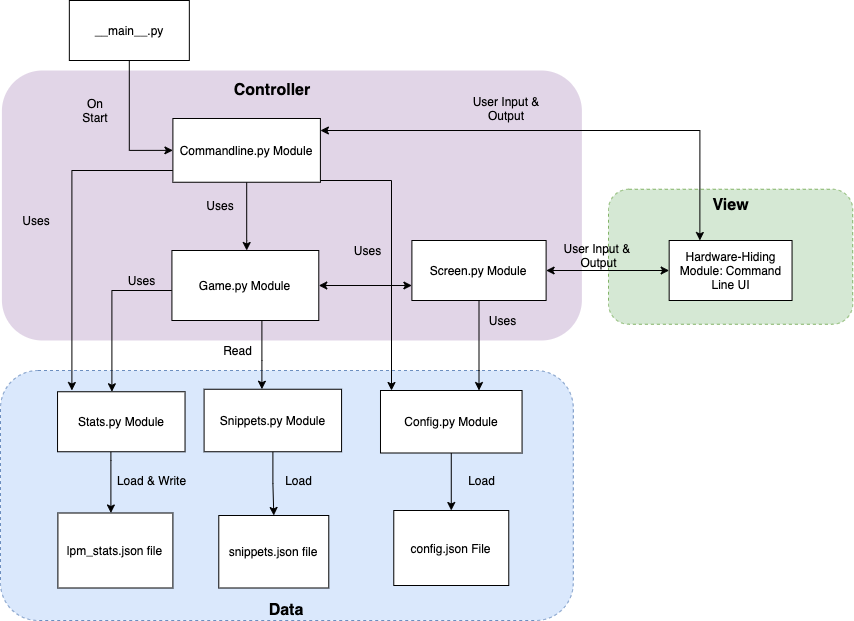
\includegraphics[scale=0.5]{3xa3_archdiagram.png}
\caption{Use hierarchy among modules}
\label{FigUH}
\end{figure}

\section{Gantt Chart}

See Gantt Chart with the testing plan at the following \href{https://gitlab.cas.mcmaster.ca/modyj/3xa3/-/tree/master/ProjectSchedule}{link}: \\

A snippet of the relevant portion of the Gantt chart can be found below:
\begin{figure}[!htbp]
\centering
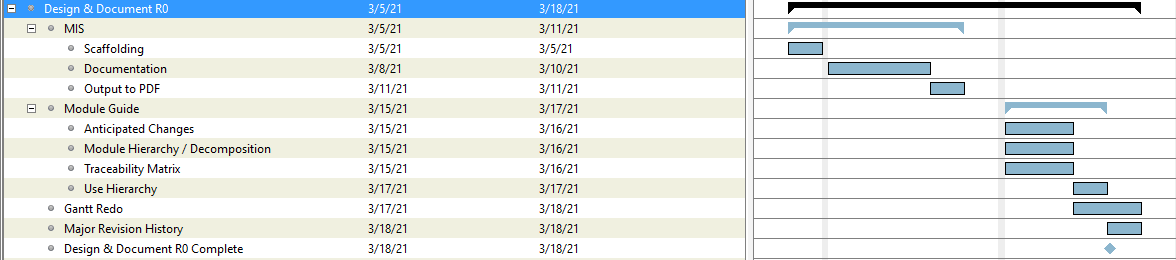
\includegraphics[scale=0.5]{MG_Gantt.png}
\caption{Gantt Chart for Design & Document Checkpoint}
\label{FigUH}
\end{figure}

%\section*{References}

%\bibliographystyle {plainnat}
%\bibliography {MG}

\end{document}
